% =============================================================================
%  Self-Paced Research Project -- Multimodal Survival Prediction
%  Template: CVPR 2026 author kit (https://github.com/cvpr-org/author-kit),
%            identical to Vorlage.pdf
%  Build:    latexmk -pdf paper.tex      (oder: pdflatex -> bibtex -> 2x pdflatex)
% =============================================================================
\documentclass[10pt,twocolumn,letterpaper]{article}

%%%%%%%%% PAPER TYPE
\usepackage[review]{cvpr}      % Review-Modus fuer die Zeilennummern am Rand ...
\toggletrue{cvprfinal}          % ... aber Autorenblock statt "Anonymous CVPR submission / Paper ID"
\ClearShipoutPicture            % ... und ohne CVPR-Kopfzeile und Paper-ID-Marken
% \usepackage[pagenumbers]{cvpr} % Final-Version ohne Zeilennummern (statt der drei Zeilen oben)

%%%%%%%%% ADDITIONAL PACKAGES (before hyperref)
\usepackage{multirow}
\usepackage{bm}
% Layout tweaks offered by the official author kit (preamble.tex) for papers close to the page limit
\usepackage{microtype}
\setlength{\abovecaptionskip}{.5em}

% hyperref as recommended by the template (cleveref is loaded by cvpr.sty)
\definecolor{cvprblue}{rgb}{0.21,0.49,0.74}
\usepackage[pagebackref,breaklinks,colorlinks,allcolors=cvprblue]{hyperref}

%%%%%%%%% PAPER ID / CONFERENCE (only shown in the review version)
\def\paperID{*****}
\def\confName{CVPR}
\def\confYear{2026}

%%%%%%%%% MATH MACROS
\newcommand{\R}{\mathbb{R}}
\newcommand{\ind}{\mathbb{I}}
\newcommand{\KL}{\mathrm{KL}}
\DeclareMathOperator{\softmax}{softmax}
\DeclareMathOperator{\diag}{diag}
\DeclareMathOperator*{\argmin}{arg\,min}
\newcommand{\pmstd}[1]{{\scriptsize$\pm$#1}}

%%%%%%%%% TITLE
\title{Multimodal Survival Prediction from Whole-Slide Images and Genomic Profiles}

%%%%%%%%% AUTHORS
\author{Elias Murr\\
University of Regensburg\\
Regensburg, Germany
}

\begin{document}
\maketitle

% =============================================================================
\begin{abstract}
Whole-slide images (WSIs) capture tumor morphology and its microenvironment, whereas genomic profiles describe the molecular drivers of cancer. Combining both promises better survival prediction but requires fusing thousands of unlabeled patch embeddings with scalar measurements under right-censored supervision. We formalize multimodal survival prediction as discrete-time survival analysis over multiple-instance bags, review the fusion strategies of MCAT, MOTCat, and SurvPath, and re-evaluate them with unimodal baselines under an identical, site-grouped 5-fold cross-validation on three TCGA cohorts (1,170 patients). On average, no fusion model outperforms a genomics-only network (C-index 0.777--0.779 \vs 0.780), and the differences between the models are smaller than the variation across folds. We trace these findings to heavy censoring, few events per fold, site-confounded outcomes, and the dominance of the glioblastoma subtype.
% TODO (eigenes Modell): 1--2 Saetze zum vorgeschlagenen Modell und seinen Ergebnissen ergaenzen.
\end{abstract}

% -----------------------------------------------------------------------------
% Figure 1 (defined here so that it appears at the top of page 2)
\begin{figure*}[t]
  \centering
  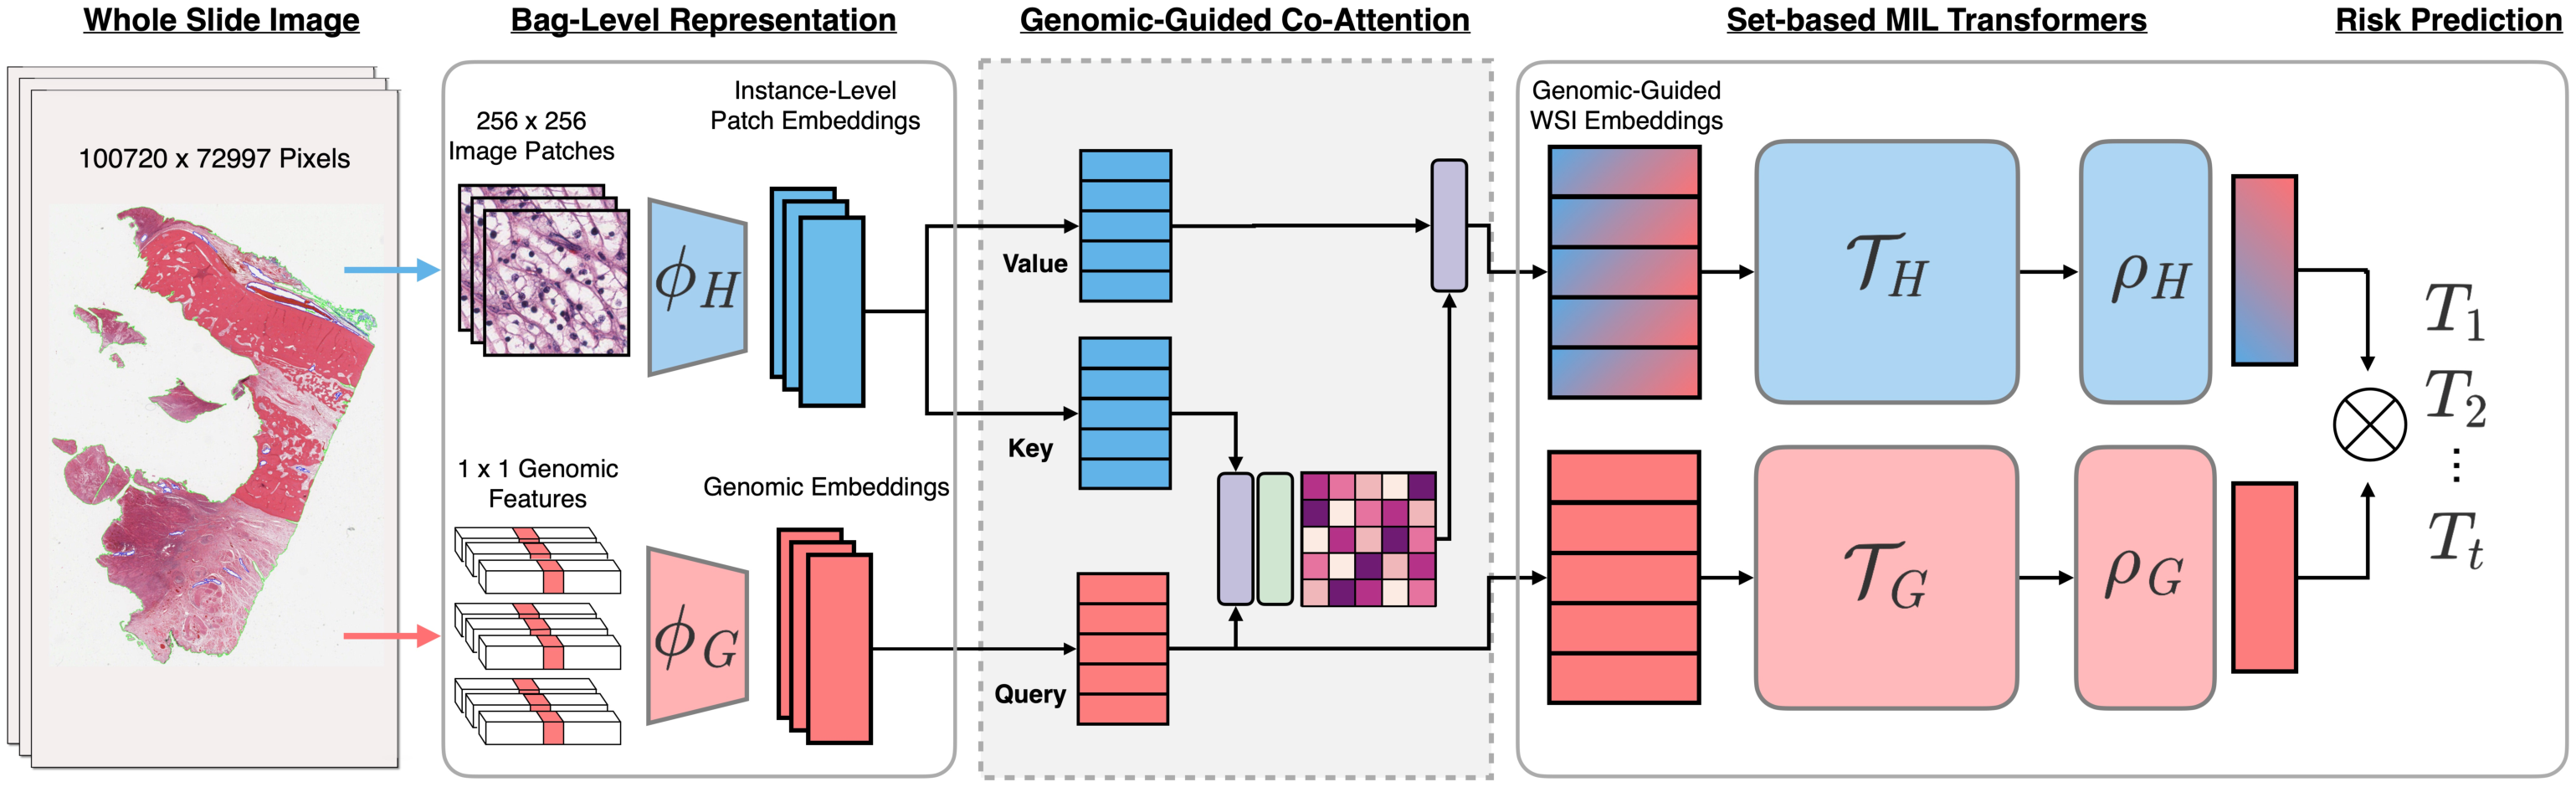
\includegraphics[width=0.7\textwidth]{figures/mcat_architecture.png}
  \caption{Multimodal survival prediction with MCAT (reproduced from~\cite{chen2021mcat}). Genomic embeddings (red) query the patch embeddings (blue) in the co-attention, and Transformers $\mathcal{T}$ with attention pooling $\rho$ process each modality before their concatenation is mapped to hazards over the intervals $T_1,\dots,T_t$.}
  \label{fig:mcat}
\end{figure*}

% =============================================================================
\section{Introduction}
\label{sec:intro}

Predicting how a cancer will progress is a central goal of precision oncology, as the prognosis guides treatment decisions. Whole-slide images (WSIs) of H\&E-stained tissue capture the morphology of the tumor and its microenvironment, whereas genomic profiles such as gene expression, mutations, and copy-number variations describe the molecular drivers of disease. Each modality shows only part of the picture, and models that integrate both often stratify patients better than unimodal ones~\cite{chen2021mcat,hemker2024healnet,raza2025ps3}.

The fusion of both modalities is, however, difficult~\cite{chen2021mcat,jaume2024survpath}. A WSI can exceed $100{,}000\times100{,}000$ pixels and is therefore processed as thousands of patch embeddings, whereas genomic measurements are $1\times1$ attributes without spatial structure, which creates a large heterogeneity gap. Since only one, often censored, outcome is known per patient and it is unknown which patches carry prognostic information, the WSI branch becomes a weakly supervised multiple-instance learning (MIL) problem~\cite{ilse2018attention}. Moreover, cohorts such as The Cancer Genome Atlas (TCGA) comprise only a few hundred patients per cancer type, and modeling all pairwise patch--gene interactions quickly becomes computationally prohibitive.

Late fusion of unimodal embeddings, for instance by a Kronecker product, cannot capture fine-grained cross-modal interactions, and early fusion by concatenation destroys the structure of the WSI bag~\cite{hemker2024healnet,raza2025ps3}. Recent models therefore let the tokens of both modalities interact through attention. MCAT~\cite{chen2021mcat} aggregates the patch embeddings with genomic queries, MOTCat~\cite{xu2023motcat} replaces this co-attention by optimal transport, and SurvPath~\cite{jaume2024survpath} fuses pathway and patch tokens in a sparse Transformer, while HEALNet~\cite{hemker2024healnet} tolerates missing modalities and PS3~\cite{raza2025ps3} adds pathology reports as a third modality.

This project addresses how gigapixel images are best fused with genomic profiles, which modality drives the prediction, and whether a model remains reliable when one modality is missing at inference time. We first formalize the pipeline from a WSI and a genomic profile to the concordance index (\cref{sec:formulation}) and contrast MCAT, MOTCat, and SurvPath (\cref{sec:fusion}). We then re-evaluate them together with unimodal baselines under an identical, site-grouped protocol on three TCGA cohorts and critically analyze the data (\cref{sec:data}).
% TODO (eigenes Modell): Beitrag des eigenen Modells ergaenzen, z.B. "Finally, we propose ... (Sec. 5)."

% =============================================================================
\section{Problem Formulation}
\label{sec:formulation}

\subsection{Discrete-time survival model}
\label{sec:survival}

Let $\mathcal{D}=\{(X_i,\mathbf{g}_i,t_i,\delta_i)\}_{i=1}^{N}$ contain for every patient a WSI $X_i$, a genomic profile $\mathbf{g}_i\in\R^{D}$, the observed time $t_i=\min(T_i,C_i)$ of death $T_i$ or censoring $C_i$ (end of follow-up), and the event indicator $\delta_i=\ind[T_i\le C_i]$. Survival analysis models the survival function $S(t\,|\,\mathbf{x})=P(T>t\,|\,\mathbf{x})$ given $\mathbf{x}=(X,\mathbf{g})$. Following MCAT and HEALNet~\cite{chen2021mcat,hemker2024healnet}, time is discretized into $K=4$ intervals $[\tau_{k-1},\tau_k)$ with $\tau_0=0$, $\tau_K=\infty$, and inner boundaries at the quartiles of the event times of the uncensored training patients, and $y_i$ denotes the interval that contains $t_i$. A network maps both modalities to logits $\mathbf{z}=f_\theta(X,\mathbf{g})\in\R^{K}$, which define the discrete hazard and survival functions
\begin{align}
  h_k &= \sigma(z_k) = P\big(T\in[\tau_{k-1},\tau_k)\,\big|\,T\ge\tau_{k-1},\mathbf{x}\big), \label{eq:hazard}\\
  S_k &= P(T\ge\tau_k\,|\,\mathbf{x}) = \textstyle\prod_{j=1}^{k}(1-h_j), \qquad S_0=1, \label{eq:survival}
\end{align}
with the logistic sigmoid $\sigma$. An uncensored patient contributes the likelihood $S_{y-1}h_y$ of surviving the first $y-1$ intervals and dying in interval $y$, whereas a censored patient contributes the probability $S_y$ of surviving interval $y$. Training therefore minimizes the negative log-likelihood $\mathcal{L}=\frac{1}{N}\sum_{i}\ell_i$~\cite{chen2021mcat,hemker2024healnet} with
\begin{equation}
  \ell_i = -\delta_i\log\big(S^{(i)}_{y_i-1}h^{(i)}_{y_i}\big)-(1-\alpha)(1-\delta_i)\log S^{(i)}_{y_i}, \label{eq:nll}
\end{equation}
where $\alpha=0.15$ down-weights the censored term. At inference, the risk score is $r_i=-\sum_{k=1}^{K}S^{(i)}_k$, so that a lower expected survival yields a higher risk.

\subsection{Whole-slide images as bags of patch tokens}
\label{sec:wsi}

As a WSI is far too large to be processed at full resolution, the tissue is segmented and tiled into $M$ non-overlapping patches at $20\times$ magnification, and a frozen encoder $\phi$ maps every patch $x_m$ to an embedding $\mathbf{h}_m=\phi(x_m)\in\R^{d}$ (\cref{fig:mcat}, left). Each slide thus becomes a bag $H=[\mathbf{h}_1,\dots,\mathbf{h}_M]^\top\in\R^{M\times d}$ of varying size with a single label, which requires a permutation-invariant aggregation. The standard choice is the gated attention pooling of ABMIL~\cite{ilse2018attention},
\begin{equation}
  a_m = \softmax_m\big(\mathbf{w}^\top[\tanh(V\mathbf{h}_m)\odot\sigma(U\mathbf{h}_m)]\big), \label{eq:abmil}
\end{equation}
where $V,U\in\R^{d_a\times d}$ and $\mathbf{w}\in\R^{d_a}$ are learned weights with a hidden dimension $d_a$. The term $\tanh(V\mathbf{h}_m)$ is a non-linear attention feature of patch $m$, the sigmoid branch $\sigma(U\mathbf{h}_m)$ gates this feature element-wise ($\odot$), and $\mathbf{w}$ maps the gated feature to a score that the softmax normalizes over all patches. The slide embedding $\bar{\mathbf{h}}=\sum_{m}a_m\mathbf{h}_m$ also serves as global pooling in MCAT and MOTCat. Our patches have $512\times512$ pixels and are encoded by CONCH~v1.5 ($d=768$).

\subsection{Genomic profiles as token sets}
\label{sec:genomics}

Genomic measurements are $1\times1$ attributes without semantic context. To obtain tokens, the $D$ attributes are grouped into $N_g$ biologically defined sets $\mathcal{B}_1,\dots,\mathcal{B}_{N_g}$, each encoded by its own small self-normalizing network (SNN) with fully connected layers, ELU activations, and alpha-dropout~\cite{chen2021mcat,jaume2024survpath}, which yields the token bag $G\in\R^{N_g\times d}$ with rows
\begin{equation}
  \mathbf{g}^{(n)}=\mathrm{SNN}_n\big(\mathbf{g}_{\mathcal{B}_n}\big)\in\R^{d}, \qquad n=1,\dots,N_g. \label{eq:genomic_tokens}
\end{equation}
MCAT and MOTCat use $N_g=6$ functional gene families such as oncogenes and tumor suppressors~\cite{chen2021mcat}, while SurvPath uses $N_P=331$ pathways. A fusion module $\Phi$ combines $H$ and $G$, and the fused tokens are pooled per modality, concatenated, and mapped to $\mathbf{z}$.

\subsection{Evaluation with the concordance index}
\label{sec:cindex}

Models are evaluated with the concordance index (C-index)~\cite{hemker2024healnet,raza2025ps3}, the fraction of comparable patient pairs whose predicted risks are ordered consistently with their survival times, where a pair is comparable if the patient with the shorter time experienced the event,
\begin{equation}
  C=\frac{\sum_{i\neq j}\delta_i\,\ind[t_i<t_j]\;\kappa(r_i,r_j)}{\sum_{i\neq j}\delta_i\,\ind[t_i<t_j]}, \label{eq:cindex}
\end{equation}
with $\kappa(r_i,r_j)=\ind[r_i>r_j]+\tfrac12\,\ind[r_i=r_j]$. A random ranking yields $C=0.5$ and a perfect one $C=1$. As every comparable pair is anchored at an observed event, the estimate rests on few pairs when events are rare.

% =============================================================================
\section{Fusion Strategies}
\label{sec:fusion}

The three models differ in which modality queries which, in how the interaction weights are normalized, and in how the genomic data are tokenized.

\subsection{MCAT: genomic-guided co-attention}
\label{sec:mcat}

MCAT~\cite{chen2021mcat} (\cref{fig:mcat}) uses the genomic tokens as queries and the patch embeddings as keys and values,
\begin{equation}
  \hat H=\softmax\!\Big(\frac{(GW_q)(HW_k)^\top}{\sqrt{d}}\Big)HW_v\in\R^{N_g\times d}. \label{eq:gca}
\end{equation}
Each row of the co-attention matrix $A=\softmax(\cdot)\in\R^{N_g\times M}$ is a distribution over all patches, so that every gene family aggregates its own ``gene-guided visual concept'' and the bag is compressed from $M$ patches to $N_g=6$ tokens at a cost of $\mathcal{O}(N_gMd)$. Two set-based Transformers then refine $\hat H$ and $G$ separately, attention pooling (\cref{eq:abmil}) yields one vector per modality, and their concatenation is classified. The interaction is asymmetric, since only the genomic tokens query, and every query is normalized independently, so that all gene families may attend to the same few patches.

\begin{figure}[t]
  \centering
  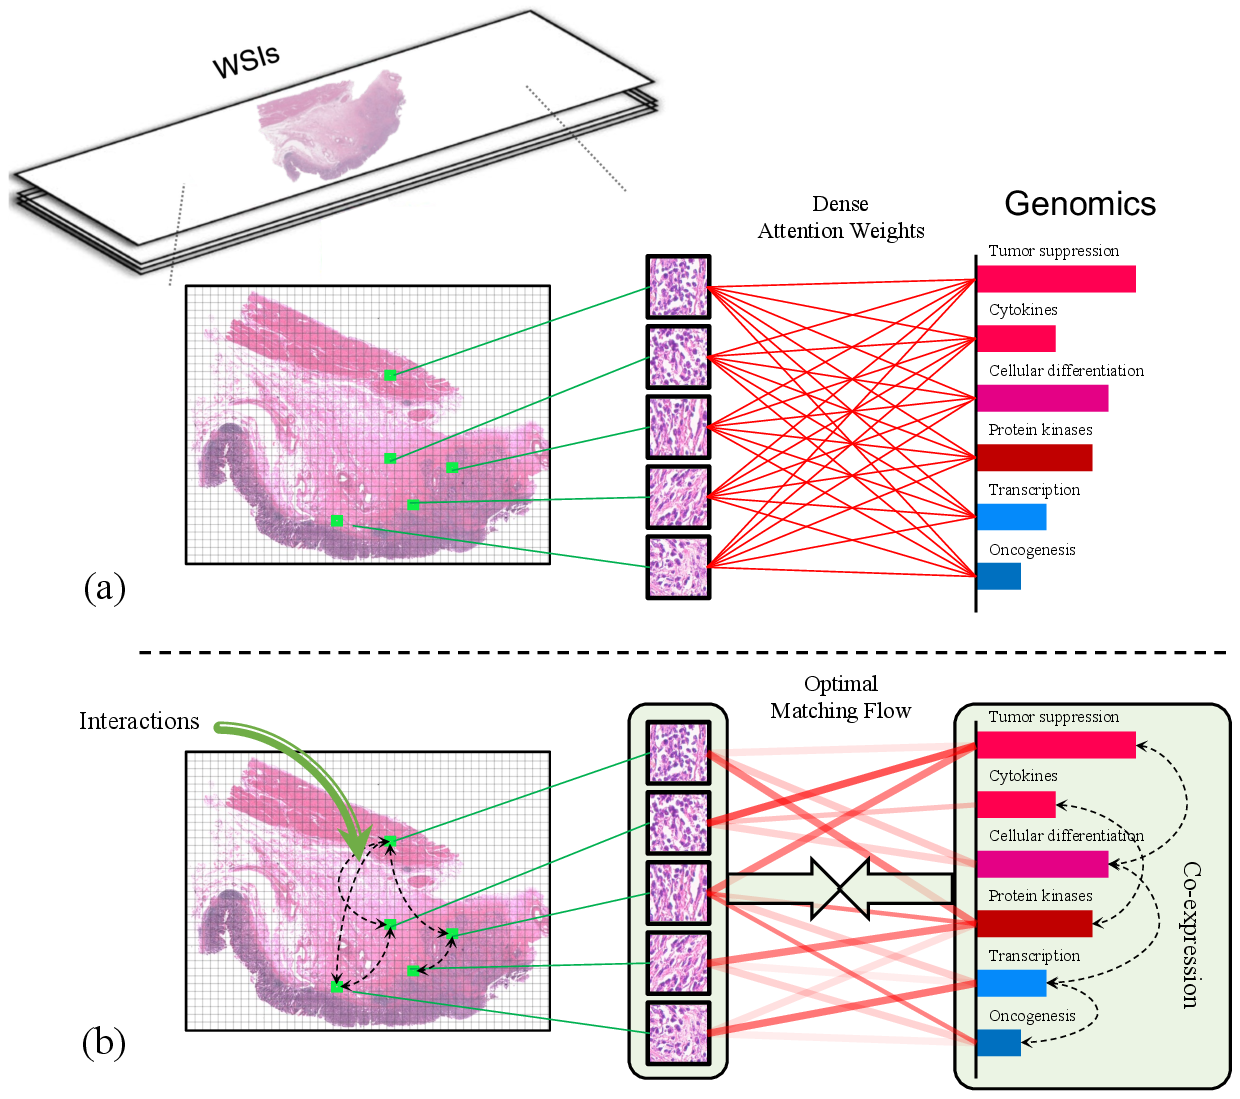
\includegraphics[width=0.6\linewidth]{figures/motcat_coattention_vs_ot.png}
  \caption{(a)~MCAT co-attention \vs (b)~MOTCat OT co-attention (reproduced from~\cite{xu2023motcat}).}
  \label{fig:motcat}
\end{figure}

\subsection{MOTCat: optimal-transport co-attention}
\label{sec:motcat}

MOTCat~\cite{xu2023motcat} keeps the MCAT architecture but replaces the softmax in \cref{eq:gca} by an optimal transport (OT) plan (\cref{fig:motcat}). OT regards the patch embeddings and the genomic tokens as two discrete distributions with uniform weights $\bm{\mu}=\tfrac{1}{M}\mathbf{1}_M$ and $\bm{\nu}=\tfrac{1}{N_g}\mathbf{1}_{N_g}$ and searches for the cheapest way to move the mass of one onto the other. Moving mass from patch $m$ to token $n$ costs $\Delta_{mn}=\|\mathbf{h}_m-\mathbf{g}^{(n)}\|_2^2$, and a transport plan $P\in\R_{+}^{M\times N_g}$ specifies the mass moved between every pair. The Kantorovich formulation minimizes the total cost over all plans that preserve both distributions,
\begin{align}
  P^\star_{\mathrm{OT}} &= \argmin_{P\in\Pi(\bm{\mu},\bm{\nu})}\;\langle P,\Delta\rangle_F=\textstyle\sum_{m,n}P_{mn}\Delta_{mn}, \label{eq:ot}\\
  \Pi(\bm{\mu},\bm{\nu}) &= \big\{P\in\R_{+}^{M\times N_g}\;\big|\;P\mathbf{1}_{N_g}=\bm{\mu},\;P^\top\mathbf{1}_M=\bm{\nu}\big\}, \notag
\end{align}
so that each patch distributes exactly its own mass over the gene families and every family receives the same total mass. Unlike the per-query softmax of MCAT, these marginal constraints couple all patches and gene families, and the plan reflects the global structure of both distributions, which MOTCat calls global structure consistency. MOTCat solves an entropically regularized and unbalanced variant, in which KL penalties with weight $\tau$ replace the hard marginal constraints, so that uninformative patches may transport less mass,
\begin{align}
  P^\star = \argmin_{P\in\R_{+}^{M\times N_g}}\; & \langle P,\Delta\rangle_F+\varepsilon\,\KL\big(P\,\|\,\bm{\mu}\bm{\nu}^\top\big)\notag\\
  & +\tau\big[\KL(P\mathbf{1}\,\|\,\bm{\mu})+\KL(P^\top\mathbf{1}\,\|\,\bm{\nu})\big]. \label{eq:uot}
\end{align}
The entropic term with weight $\varepsilon$ makes the problem strictly convex, and its solution $P^\star=\diag(\mathbf{u})\,\mathcal{K}\diag(\mathbf{v})$ with the kernel $\mathcal{K}=\exp(-\Delta/\varepsilon)\odot\bm{\mu}\bm{\nu}^\top$ is found by Sinkhorn--Knopp iterations, which alternately update $\mathbf{u}\leftarrow(\bm{\mu}\oslash\mathcal{K}\mathbf{v})^{\eta}$ and $\mathbf{v}\leftarrow(\bm{\nu}\oslash\mathcal{K}^\top\mathbf{u})^{\eta}$ with element-wise division $\oslash$ and $\eta=\tau/(\tau+\varepsilon)$ and recover the exact marginals of \cref{eq:ot} for $\tau\to\infty$. The WSI tokens are then aggregated as $\hat H=P^{\star\top}H$. Since OT on more than $10^4$ patches is expensive, MOTCat solves it on random micro-batches of $m$ patches and averages losses and risks (here $m=4096$, $\varepsilon=0.1$, $\tau=0.5$).

\subsection{SurvPath: pathway--histology Transformer}
\label{sec:survpath}

SurvPath~\cite{jaume2024survpath} tokenizes the transcriptome into $N_P=331$ pathways from Reactome and the MSigDB Hallmarks, each encoded from its member genes by its own SNN (\cref{eq:genomic_tokens}), which yields biologically interpretable tokens $X_P$. Together with the projected patch tokens $X_H$, they form one sequence for a Transformer layer whose $(N_P+M)^2$ attention matrix would be dominated by the patch--patch block, which SurvPath therefore masks,
\begin{equation}
  \hat X = \sigma_{\mathrm{row}}\Big(\tfrac{1}{\sqrt{d}}\begin{pmatrix}Q_PK_P^\top & Q_PK_H^\top\\ Q_HK_P^\top & -\infty\end{pmatrix}\Big)\begin{pmatrix}V_P\\ V_H\end{pmatrix}, \label{eq:survpath}
\end{equation}
where $\hat X=[\hat X_P;\hat X_H]$ stacks the updated pathway and patch tokens and $\sigma_{\mathrm{row}}$ is the row-wise softmax. Pathways thus attend to pathways and patches and patches attend to pathways, which reduces the memory to $\mathcal{O}(N_P^2+2N_PM)$, before both token types are mean-pooled and concatenated. Unlike MCAT and MOTCat, SurvPath fuses bidirectionally, keeps all patch tokens, and uses pathway-resolved transcriptomics only, but like them it ignores patch--patch interactions and cannot predict when one modality is missing.

% =============================================================================
\section{Dataset and Baseline Evaluation}
\label{sec:data}

\begin{figure}[t]
  \centering
  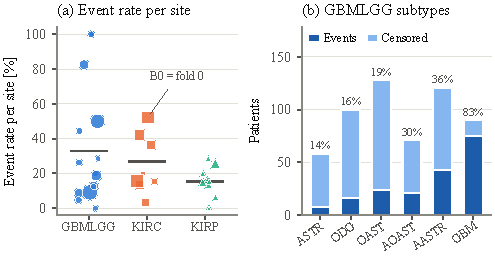
\includegraphics[width=\linewidth]{figures/dataset_overview.pdf}
  \caption{Cohort analysis. (a)~Event rate per tissue source site with at least ten patients (marker area $\propto$ patients, bar: cohort rate), where site B0 alone forms KIRC test fold~0. (b)~Patients, events, and event rates per GBMLGG subtype (GBM: glioblastoma, (A)ASTR: (anaplastic) astrocytoma, ODG: oligodendroglioma, (A)OAST: (anaplastic) oligoastrocytoma).}
  \label{fig:dataset}
\end{figure}

\subsection{Cohorts and protocol}
\label{sec:cohorts}

We use the TCGA cohorts of glioblastoma and lower-grade glioma (GBMLGG), clear-cell renal cell carcinoma (KIRC), and papillary renal cell carcinoma (KIRP) with one diagnostic slide, the overall survival (OS), and the censorship status per patient. MCAT and MOTCat receive the RNA-seq, mutation, and CNV features distributed with MCAT in six gene families, whereas SurvPath and the genomics-only baselines receive pan-cancer normalized RNA-seq from UCSC Xena as in SurvPath~\cite{jaume2024survpath} for the 4,917 genes of 330 non-empty pathways. \Cref{tab:cohorts} and \cref{fig:dataset} summarize the 1,170 patients.

All models share one 5-fold cross-validation whose folds are grouped by tissue source site to mitigate batch artifacts, as in SurvPath~\cite{jaume2024survpath}, and stratified by event status and time interval, keeping the most balanced of 1,000 random assignments with at least five events per fold. Interval boundaries and z-scoring are fitted on the training folds only. All networks are trained for 20 epochs with AdamW (learning rate $2\times10^{-4}$, weight decay $10^{-5}$, cosine schedule, effective batch size 32), and we report the final-epoch C-index, so the test fold is never used for model selection. The unimodal baselines are ABMIL~\cite{ilse2018attention} and TransMIL~\cite{shao2021transmil} on the WSIs and an SNN~\cite{chen2021mcat} and a two-layer MLP on the pathway genes.

\begin{table}[t]
  \centering
  \footnotesize
  \setlength{\tabcolsep}{3.2pt}
  \begin{tabular}{@{}lccc@{}}
    \toprule
                                       & GBMLGG & KIRC & KIRP\\
    \midrule
    Patients / events                  & 568 / 187 & 343 / 92 & 259 / 40\\
    Censored                           & 67.1\% & 73.2\% & 84.6\%\\
    Median follow-up$^\dagger$ [months]& 28 & 49 & 27\\
    Tissue source sites                & 35 & 17 & 31\\
    Events per test fold               & 24--51 & 11--35 & 7--9\\
    Patches per WSI (median)           & 2,338 & 3,902 & 3,543\\
    Gene-family RNA/mut./CNV           & 1,544/11/18 & 1,556/5/137 & 1,557/5/0\\
    \bottomrule
  \end{tabular}
  \caption{Cohort statistics. $^\dagger$Reverse Kaplan--Meier estimate.}
  \label{tab:cohorts}
\end{table}

\begin{table}[t]
  \centering
  \footnotesize
  \setlength{\tabcolsep}{2.4pt}
  \begin{tabular}{@{}llcccc@{}}
    \toprule
    & Model & GBMLGG & KIRC & KIRP & Avg.\\
    \midrule
    \multirow{2}{*}{WSI}   & ABMIL             & 0.750\pmstd{.071} & 0.697\pmstd{.088} & 0.757\pmstd{.105} & 0.735\\
                           & TransMIL          & 0.755\pmstd{.067} & 0.708\pmstd{.062} & 0.749\pmstd{.096} & 0.737\\
    \midrule
    \multirow{2}{*}{Gen.}  & SNN               & 0.818\pmstd{.033} & 0.702\pmstd{.063} & \textbf{0.820}\pmstd{.124} & \textbf{0.780}\\
                           & MLP               & \textbf{0.830}\pmstd{.043} & 0.705\pmstd{.054} & 0.791\pmstd{.141} & 0.775\\
    \midrule
    \multirow{3}{*}{Both}  & MCAT              & 0.787\pmstd{.036} & \textbf{0.734}\pmstd{.046} & 0.818\pmstd{.120} & 0.779\\
                           & MOTCat            & 0.788\pmstd{.039} & 0.725\pmstd{.034} & 0.818\pmstd{.135} & 0.777\\
                           & SurvPath          & 0.826\pmstd{.049} & 0.718\pmstd{.048} & 0.789\pmstd{.127} & 0.777\\
    \bottomrule
  \end{tabular}
  \caption{C-index (mean\,$\pm$\,std over the five site-grouped test folds, final epoch); Avg.: mean over cohorts; best per column in bold.}
  \label{tab:results}
\end{table}

\subsection{Baseline results}
\label{sec:results}

The WSI-only models in \cref{tab:results} reach an average C-index of 0.735--0.737 and remain clearly below the genomics-only models (0.775--0.780). The fusion models MCAT, MOTCat, and SurvPath (0.777--0.779) do not exceed the SNN on average, and only on KIRC do all three beat the best unimodal model, by up to 0.026 for MCAT. The prediction is thus driven predominantly by the genomic modality, in line with the modality dominance discussed in HEALNet~\cite{hemker2024healnet} and PS3~\cite{raza2025ps3}. Moreover, the gaps between the fusion models of at most 0.04 are smaller than the fold-wise standard deviations of up to 0.14, which depend more on the fold than on the model, as all seven networks score 0.55--0.64 on KIRP fold~2 but 0.80--0.96 on fold~0.

\subsection{Critical assessment of the dataset}
\label{sec:critique}

Several properties of the data explain these observations. KIRP has 84.6\% censored patients and only 7--9 events per test fold, so that each fold's C-index rests on only 163--268 comparable pairs (\cref{eq:cindex}) and even the interval boundaries stem from about 32 training events, which makes the model ranking on KIRP unreliable.

Overall survival counts deaths from any cause, and a median follow-up of 27--49 months is short for slowly progressing lower-grade glioma or papillary renal cell carcinoma, which is why SurvPath and PS3 predict disease-specific survival~\cite{jaume2024survpath,raza2025ps3}, available here only for KIRP.

Outcomes are also confounded with the tissue source site, as the event rate of sites with at least ten patients ranges from 3\% to 52\% in KIRC and from 0\% to 100\% in GBMLGG (\cref{fig:dataset}a). Site-grouped folds prevent WSI models from exploiting site-specific staining as a proxy for risk but are heterogeneous, as KIRC fold~0 contains only site B0 with 35 of 92 events and is the hardest fold for all WSI-based models.

In GBMLGG, the 90 glioblastoma patients form 16\% of the cohort but account for 40\% of the events, with an event rate of 83\% compared with 14--36\% for the lower-grade subtypes (\cref{fig:dataset}b). Much of the achievable concordance thus likely reflects the coarse separation of glioblastoma from lower-grade glioma, not differences within subtypes.

Finally, KIRP lacks CNV features, only 5--11 mutation features fall into the six gene families, and the different genomic inputs of MCAT/MOTCat and SurvPath confound the comparison of architectures with that of input representations. Bag sizes vary between 10 and 11,102 patches, one slide per patient is used, and our CONCH features differ from those of the original works~\cite{chen2021mcat,xu2023motcat,jaume2024survpath}, so absolute values are not comparable with published results.

% =============================================================================
% 5. Proposed method  (folgt -- eigener Modellvorschlag)
% =============================================================================

{
    \small
    \bibliographystyle{ieeenat_fullname}
    \bibliography{references}
}

\end{document}
